%%% DOCUMENT BEGIN

\documentclass{article}

\usepackage[utf8]{inputenc}

\usepackage{geometry}
\geometry{a4paper}

\usepackage{graphicx}

%%% PACKAGES
\usepackage{booktabs} % for much better looking tables
\usepackage{array} % for better arrays (eg matrices) in maths
\usepackage{paralist} % very flexible & customisable lists (eg. enumerate/itemize, etc.)
\usepackage{verbatim} % adds environment for commenting out blocks of text & for better verbatim
\usepackage{subfig} % make it possible to include more than one captioned figure/table in a single float

%%% HEADERS & FOOTERS
\usepackage{fancyhdr} % This should be set AFTER setting up the page geometry
\pagestyle{fancy} % options: empty , plain , fancy
\renewcommand{\headrulewidth}{0pt} % customise the layout...
\lhead{}\chead{}\rhead{}
\lfoot{}\cfoot{\thepage}\rfoot{}

%%% SECTION TITLE APPEARANCE
\usepackage{sectsty}
\allsectionsfont{\sffamily\mdseries\upshape}

%%% ToC (table of contents) APPEARANCE
\usepackage[nottoc,notlof,notlot]{tocbibind} % Put the bibliography in the ToC
\usepackage[titles,subfigure]{tocloft} % Alter the style of the Table of Contents
\renewcommand{\cftsecfont}{\rmfamily\mdseries\upshape}
\renewcommand{\cftsecpagefont}{\rmfamily\mdseries\upshape} % No bold!


%%% END Article customizations


%%%%%%%%%%%%%%%%%%%%%%%%%
%%%          Fill in the title details                      %%%

\def \thetitle {INF-1101 Datastrukturer og algoritmer}
\def \thesubtitle {Assignment 1 - Set ADT}
\def \theauthor {Kandidatnummer 0}
\def \pagecount {3}

%%%%%%%%%%%%%%%%%%%%%%%%%

%\pagestyle{fancy}
\pagestyle{fancyplain} % options: empty , plain , fancy
\renewcommand{\headrulewidth}{1pt} % customise the layout...
\renewcommand{\footrulewidth}{0pt}
\lhead{\fancyplain{}{\thetitle{} -- \thesubtitle{}}}\chead{}\rhead{\fancyplain{}{\theauthor{}}}
\lfoot{}\cfoot{Page {\thepage} of \pagecount}\rfoot{}

\begin{document}

%%% TITLE PAGE

\begin{titlepage}
\begin{center}



\textsc{\\[3.5cm] \huge University of Tromsø}\\[1.5cm]

\textsc{\LARGE \thetitle}\\[0.5cm]

\textsc{\Large \thesubtitle}\\[1.5cm]

\LARGE{\theauthor} \\[0.5cm] \large{Department of Computer Science}



\vfill
{\large \today}

\end{center}
\thispagestyle{empty}
\end{titlepage}

\newpage{}


%%% TABLE OF CONTENTS

%\tableofcontents


\newpage{}

%%% DOCUMENT BODY

%%% Set counter to 1
\setcounter{page}{1}

\section{Introduction}

Short introduction to the assignment, motivation and expected results.

\subsection{Requirements}

Outline the detailed requirements specified in the assignment text.

\begin{itemize}

\item First requirement
\item Next requirement
\item etc.

\end{itemize}


\section{Technical Background}

Which topics are covered in this assignment. Should be short and cover the necessary topics without mentioning your specific implementation and design.

\subsection{Data Structures}

Since this is a course in algorithms, so it might be a good idea to cover the basic data-structures(e.g. lists and trees). 

Figure \ref{fig:ackseq} shows how you can add figures to the report. And below is the LaTeX syntax for adding a figure:

% Verbatim prints the text without formatting
\begin{verbatim}
\begin{figure}
\begin{center}
\fbox{\includegraphics[width=177px]
{source.png}}
\end{center}
\caption{Description}\label{fig:descriptiveLabel}
\end{figure}
\end{verbatim}

% An example figure
\begin{figure}[h]
\begin{center}
\fbox{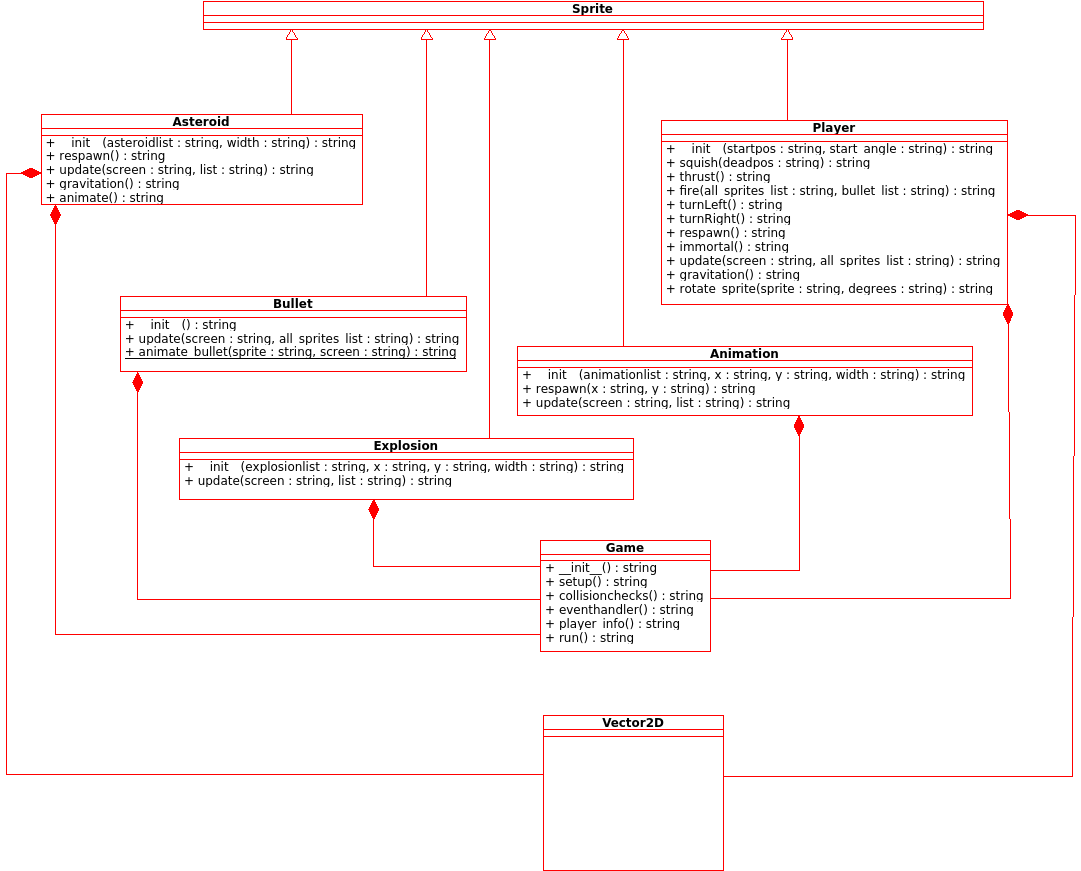
\includegraphics[width=177px]
{classdiagram.png}}
\end{center}
\caption{A binary search tree}\label{fig:ackseq}
\end{figure}

\subsection{Another section}

Some more information

\section{Design}

How did you solve the assignment? Describe the architecture and any design choices you've made. Show figures of the proposed architecture.

\section{Implementation}

How did you implement, deploy and run your application? No need to refer to actual lines of code.

\section{Discussion}

Any advantages or disadvantages with your design?

\subsection{Evaluation}

This section should contain relevant graphs and test results.

\section{Conclusion}

Sum up by restating the problem and solution. Follow up with a brief summary of the solution along with lessons learned.


%%% BIBLOGRAPHY

\newpage{}


\begin{thebibliography}{9}

\bibitem{coursebook}
 Robert Sedgewick 
  \emph{Algorithms in C - parts 1-4}.
  Addison-Wesley Publishing Company,
  3. Edition,
  1998.

\end{thebibliography}

\end{document}
